\documentclass{ieeeaccess}
\usepackage{cite}
\usepackage{amsmath,amssymb,amsfonts}
\usepackage{algorithmic}
\usepackage{graphicx}
\usepackage{textcomp}
\usepackage{booktabs}
\usepackage{flafter}
\usepackage{url}
\usepackage{hyperref}
\usepackage{xurl}
\usepackage{threeparttable}
\usepackage{tabularx}
\setcounter{topnumber}{2}
\setcounter{bottomnumber}{2}
\setcounter{totalnumber}{4}
\renewcommand{\topfraction}{0.95}
\renewcommand{\bottomfraction}{0.95}
\renewcommand{\textfraction}{0.05}
\renewcommand{\floatpagefraction}{0.9}

\usepackage{bm}
\makeatletter
\AtBeginDocument{\DeclareMathVersion{bold}
\SetSymbolFont{operators}{bold}{T1}{times}{b}{n}
\SetSymbolFont{NewLetters}{bold}{T1}{times}{b}{it}
\SetMathAlphabet{\mathrm}{bold}{T1}{times}{b}{n}
\SetMathAlphabet{\mathit}{bold}{T1}{times}{b}{it}
\SetMathAlphabet{\mathbf}{bold}{T1}{times}{b}{n}
\SetMathAlphabet{\mathtt}{bold}{OT1}{pcr}{b}{n}
\SetSymbolFont{symbols}{bold}{OMS}{cmsy}{b}{n}
\renewcommand\boldmath{\@nomath\boldmath\mathversion{bold}}}
\makeatother

\def\BibTeX{{\rm B\kern-.05em{\sc i\kern-.025em b}\kern-.08em
    T\kern-.1667em\lower.7ex\hbox{E}\kern-.125emX}}

% ============================================================================
% Revised manuscript for Access-2026-52910.
% This file is a separate working copy. The submitted access.tex is untouched.
% Numbers are frozen from the revision artifacts; tables and figures are
% generated from the committed aggregate files.
% ============================================================================

\graphicspath{{figures/}{./}}

\begin{document}

% Volume and year are updated for the resubmission; the DOI is assigned by
% IEEE Access production and is left as a placeholder for review.
\year{2026}
\vol{14}
\doi{10.1109/ACCESS.2026.XXXXXXX}

\title{When Feedback Gains Are Borrowed: Procedure Overlap, Calibration, and the Limits of Similarity-Based Evaluation in RAG for IT Support}
\author{\uppercase{Domen Jer\v{s}ek}\authorrefmark{1},
\uppercase{Bla\v{z} Ka\v{z}i\v{c}}\authorrefmark{1}, AND \uppercase{Klemen Kenda}\authorrefmark{1}}

\address[1]{ARTIFICIAL INTELLIGENCE DEPARTMENT - E3, Jo\v{z}ef Stefan Institute, Ljubljana, Slovenia
(e-mail: domenjersek@gmail.com, blaz.kazic@ijs.si, klemen.kenda@ijs.si). ORCID: D. Jer\v{s}ek 0009-0009-1822-8277, B.
Ka\v{z}i\v{c} 0000-0002-1335-7960, K. Kenda 0000-0002-4918-0650.}

\tfootnote{This work has received funding from the European Union's Horizon Europe research
and innovation programme under grant agreement No~101120218 (HumAIne). Views and opinions
expressed are however those of the author(s) only and do not necessarily reflect those of the
European Union or the granting authority. Neither the European Union nor the granting authority
can be held responsible for them. The authors acknowledge the use of large language models for
language editing and for the simulated feedback scoring described in the paper; all conceptual
frameworks, analyses, and interpretations remain the sole responsibility of the authors.}

\markboth
{D. Jer\v{s}ek \headeretal: When Feedback Gains Are Borrowed}
{D. Jer\v{s}ek \headeretal: When Feedback Gains Are Borrowed}

\corresp{Corresponding author: Domen Jer\v{s}ek (e-mail: domenjersek@gmail.com).}

\begin{abstract}
Feedback from historical ticket--candidate pairs is widely used to rerank retrieval
candidates in retrieval-augmented generation for IT support. We show that the
measured benefit depends less on the judge than on whether evaluation tickets share
procedures with the historical base. Using 1,595 enterprise tickets, we rebuild the
evaluation so that retrieval, feedback and priors use only the training partition,
and compare familiar-procedure, duplicate-removed and strict
procedure-disjoint regimes. Under strict disjointness, blind feedback no longer
harms ($-0.044$ to $+0.001$) and the conditioned effect is small ($+0.009$),
metric-dependent and not robust to multiplicity correction. A reply-similarity baseline that uses no LLM judge matches the LLM judge only
when procedures overlap. A blinded expert
assessment of 105 tickets does not confirm a difference on new procedures; on familiar
procedures the expert's apparent preference for feedback is explained by answer
length, and expert and cosine metric disagree. Gains reported on overlapping splits
are therefore partly borrowed from procedure overlap; calibration removes harm
without a confirmed gain; and similarity to one recorded reply is not procedural
correctness.
\end{abstract}

\begin{keywords}
Feedback reranking, information retrieval, large language models,
retrieval-augmented generation, evaluation validity, ticket resolution.
\end{keywords}

\titlepgskip=-21pt

\maketitle


% ============================================================================
\section{Introduction}
\label{sec:introduction}
\PARstart{S}{upport} organizations answer thousands of tickets, and many of them
restate problems that have been solved before. Retrieval-augmented generation
(RAG) makes reuse natural: retrieve the most similar historical tickets and let a
language model write the first reply from their resolutions
\cite{b1,b31}. The implicit assumption is that textual similarity tracks
procedural similarity. It often does not.

Enterprise ticket streams make this failure common and its measurement hard.
Procedures are long-tailed and organized by team and intent, so many tickets have
few close historical neighbours, while the closest neighbours may belong to a
different procedure that shares vocabulary. Unlike search or recommendation, the
domain has no click stream: the only observable signal of usefulness is whether a
procedure matches the one that resolved the ticket. We therefore simulate the
missing feedback with large language model (LLM) judges and treat the judge's
information as an experimental variable.

A random-split evaluation of this pipeline reveals a striking pattern. The same
fine-scope reranking improves generated first replies when the judge sees the
historical resolution, and harms them when the judge sees only the ticket. That contrast is real, but it is not yet an answer to the question a
deployment team faces. A random split lets evaluation tickets share a
procedure, a reply template, or a near-duplicate with the historical base. A gain
measured there may describe the data regime as much as the feedback method.

This paper asks the prior question: \emph{does any of the gain survive when the
evaluation ticket does not share a procedure or a reply template with the
historical base?} To answer it, we rebuild the evaluation around three data
regimes. In the \emph{familiar} regime the historical base may contain a ticket
with the same procedure or reply template, as in a random split. In the
\emph{duplicate} regime tickets with an identical normalized full reply or an
identical title and subcategory are kept out of the evaluation side. In the
\emph{strict} regime tickets that even share the first 300 reply characters are
kept apart. Every regime uses a training-only candidate index, training-only BM25
statistics, feedback rows with both endpoints in training, and priors estimated
from exactly those rows. The strict panel is the primary control; the familiar
panel reproduces the random-split setting.

The answer changes the reading of the random-split result. Under strict disjointness,
blind feedback no longer harms: the familiar-panel effect of $-0.0444$ becomes
$+0.0008$ (p=.86). The conditioned effect remains small ($+0.0093$), its cosine
interval excludes zero but the rank test is marginal (p=.066), ROUGE-L is not
significant, and the effect lies below the study's 80\,\% minimum detectable
effect (0.0103). A reply-similarity baseline that uses no LLM judge matches
the conditioned judge on the familiar panel ($+0.0143$ versus $+0.0105$) but not
on the strict panel ($+0.0026$ versus $+0.0093$). The pattern is consistent with a
simple explanation: part of the measured benefit on overlapping data is borrowed
from procedures and reply templates that the evaluation ticket shares with
history.

A blinded expert assessment of 105 changed pairs completes the picture. On new
procedures the expert does not confirm a difference between baseline and feedback (strict
blind $-0.030$ $[-0.121,+0.061]$; strict conditioned $0.000$
$[-0.088,+0.088]$). On familiar procedures the expert prefers feedback by $+0.147$
$[0.000,+0.294]$, but the feedback replies are 173 characters longer, the
preference tracks length (Spearman $+0.63$), and among length-matched pairs the
effect is exactly zero. On that arm the expert and the cosine metric point in
opposite directions (expert $+0.147$, automatic $-0.088$), which is direct
evidence that similarity to one recorded reply is not procedural correctness. The
study is a validity check, not a confirmatory trial: one expert has completed the
sample, the second is in progress, and the arms contain only 2--7 discordant pairs.

The paper makes four contributions.

\begin{enumerate}
\item \textbf{The data regime is the experimental variable.} We define versioned
structural groups over identical full replies or identical title and subcategory,
and a conservative prefix variant; assign whole groups to train, dev and eval; and
restrict retrieval, BM25 statistics, feedback rows and scope priors to the same
allowed history. A combined-hash split is shown not to be procedure-disjoint:
12.8\,\% of its evaluation tickets share an identical full reply and 53.3\,\%
share a 300-character reply opening with training. Five
group-aware splits are generated for each rule.
\item \textbf{The repair is decomposed.} A one-factor-at-a-time dev ablation varies
the tuned Laplace baseline, empirical-Bayes centering, pool-relative scaling, scope
and backoff under a matched selection budget. The inherited legacy cell ranks 23rd
of 25 Laplace configurations on the strict panel. With one feedback configuration,
the gain is similar across dense, BM25 and hybrid retrieval; the claim that
stronger retrieval reduces the benefit is a scaling artefact.
\item \textbf{The calibrated outcome is a harm removal, not a confirmed gain.} On
strict history, the blind harm disappears, the conditioned effect is small and
metric-dependent, and no cell survives multiplicity correction with a magnitude
above the design's detection threshold. A reply-similarity prior that uses no LLM
judge is competitive only where procedure overlap remains.
\item \textbf{An expert validity check separates procedure from similarity.} The
blinded assessment does not confirm a difference on new procedures; on familiar procedures
the apparent preference for feedback is explained by answer length, and expert and
cosine judgements diverge. This is direct evidence that the automatic metric and
the human judgement capture different things, and that neither is a clean
criterion.
\end{enumerate}

This article re-uses the retrieval and generation pipeline of our prior
conference work \cite{b31,b32} as a fixed component; the data-regime control, the
split audit, the controlled repair, the reply-similarity baseline, the
matched-retriever comparison, the statistical sensitivity analysis and the expert
evaluation are new. No text, tables or figures from the conference papers are
reused. Section~\ref{sec:related} positions the work and details the relationship;
Section~\ref{sec:data} defines the data regimes; Section~\ref{sec:method} the
method; Sections~\ref{sec:baseline}--\ref{sec:validation} the results; and
Sections~\ref{sec:discussion} and~\ref{sec:conclusion} the discussion and
conclusion.


% ============================================================================
\section{Related Work}
\label{sec:related}

\subsection{Retrieval-augmented generation and reranking}
Retrieval-augmented generation conditions a generator on retrieved evidence
\cite{b1}, and dense bi-encoders such as Sentence-BERT made semantic retrieval
practical \cite{b2,b28}; Facebook AI Similarity Search (FAISS) provides the
nearest-neighbour infrastructure at scale \cite{b3}. Sparse retrieval remains a
strong baseline \cite{b4}, hybrid fusion by reciprocal rank fusion (RRF) is a
common robustness measure \cite{b5}, and cross-encoder reranking improves the top
of the ranking at higher cost \cite{b6}. Dense passage retrieval established the
two-stage recipe we follow \cite{b7}. All of this machinery is fixed in our study;
the object of study is the feedback signal applied on top of it. Reranking matters
most where the first stage is imperfect: a cross-encoder sees the query and
candidate jointly and can correct ordering errors that a bi-encoder cannot
\cite{b6}. RAG evaluation, in turn, separates retrieval quality from answer
quality \cite{b1,b40,b41}, a distinction that our proxy-versus-generated
divergence reproduces.

\subsection{Learning to rank from feedback signals}
Relevance feedback is one of the oldest ideas in information retrieval:
Rocchio-style query modification moves the query toward relevant documents
\cite{b8}, and relevance-based language models estimate a query model from feedback
documents \cite{b9}. Learning-to-rank inherits the same assumption---that logged
interactions carry usable relevance signal. Two questions that this literature
often leaves implicit are the ones we make explicit: \emph{what the feedback source
knows}, and \emph{how its evidence is converted into a score}. Feedback in
recommender systems, for instance, is known to carry popularity and base-rate bias
\cite{b10}; we show an analogous pathology in judge-driven ticket feedback,
identify its arithmetic cause, and repair it without labels. A second strand studies
implicit feedback and click models, where exposure and position bias must be
corrected before interactions can be treated as relevance \cite{b34,b37}. Our
setting removes exposure bias by judging every candidate in a pool, but it
introduces a different pathology: the judge's evidence is sparse and zero-heavy,
and the score construction amplifies that sparsity.

\subsection{LLM-as-judge validity}
Large language models are increasingly used as relevance and quality judges
\cite{b11,b12,b35,b36}. Their known failure modes include position bias, verbosity
bias, and self-preference \cite{b13,b14}. Our protocols differ from ordinary LLM
judging in one decisive respect: the conditioned judge receives the historical
resolution of the training query, which makes it a \emph{resolution-informed}
judge and an upper bound on what resolution-aware evidence can buy. It is
deployable for historical pairs: both tickets in a historical pair have known
resolutions, so the conditioned votes can be precomputed for the historical base.
At inference on a new ticket, however, no resolution exists yet, so only blind
votes can be generated for that ticket. We therefore report both protocols side by side, state exactly
what each judge and metric sees, and add an expert assessment of the generated
answers (Section~\ref{sec:expert}). Judge agreement is usually reported in
aggregate; the random-split analysis found low per-ticket agreement between its
independent judge and the automatic metric, which we treat as a limitation of the
measurement rather than as evidence against the aggregate signal.

\subsection{Calibration, selective prediction, and abstention}
Converting scores into calibrated quantities is a classical problem
\cite{b15,b16,b17}, and empirical Bayes provides a standard way to stabilize rate
estimates built from few observations \cite{b18,b19,b38,b39}. Decision theory
prescribes abstention when expected utility is negative \cite{b20}; selective
prediction operationalizes this for classifiers \cite{b21}, and cost-sensitive
learning makes the trade-off explicit \cite{b22}. Our gate is a selective predictor
over tickets. Bayesian smoothing with a Beta or Dirichlet prior is standard in
language modelling and information retrieval \cite{b18,b19}; our empirical-Bayes
lift is a direct application of that idea to a per-candidate rate estimated from
very few votes. We do not claim the smoother as a methodological contribution; the
contribution is the demonstration that it removes harm without creating a confirmed
gain once procedure overlap is controlled.

\subsection{Relationship to prior work}
\label{sec:prior}
Two prior papers by the authors are the direct starting point. \cite{b31}
introduced the retrieval and generation pipeline for first-reply generation;
\cite{b32} added LLM-judge feedback as a retrieval modifier and reported an
exploratory, conditioned-only analysis on 250 leave-one-out queries with a
different judge, in which no always-on method was significant and retrieval-score
gates were indistinguishable from always-on. The present article re-uses the
pipeline and the legacy lift formula as fixed components. Its contribution is
different: it treats the data regime as the experimental variable, audits the
combined-hash split, restricts retrieval, feedback and priors to an allowed history,
isolates the components of the calibration repair, adds a reply-similarity
baseline that uses no LLM judge and a matched-retriever comparison, and reports a blinded expert
assessment of procedural correctness. Table~\ref{tab:prior} compares the studies
side by side. No text, tables or figures are reused; the overlap is limited to the
cited background, and the connection is disclosed here as required for expanded
conference versions.

\Table[!btp](width=\textwidth){Relationship to the authors' prior conference
papers and to the random-split baseline. This article shares the
corpus and the base pipeline; the data-regime control, split audit, controlled
repair, reply baseline, matched retrievers, statistical sensitivity analysis and
expert evaluation are new.\label{tab:prior}}{
\scriptsize
\begin{tabularx}{\textwidth}{@{}p{0.15\textwidth}>{\raggedright\arraybackslash}X>{\raggedright\arraybackslash}X>{\raggedright\arraybackslash}X>{\raggedright\arraybackslash}X@{}}
\toprule
 & SIKDD 2025 & SIKDD 2026 & Random-split baseline & This article \\
\midrule
Role & Retrieval + generation pipeline & Exploratory feedback-aware retrieval & Protocol contrast on a random split & Data regime and measurement validity \\
Corpus & Enterprise IT tickets & 1,596 tickets, 37 teams & 1,595 tickets, 37 teams, 17 classes & Same 1,595; canonical IDs unchanged \\
Evaluation queries & --- & 250 leave-one-out & Random 878/319/398; 390 combined-hash eval & History-only 398/398/427 \\
Judge & --- & gpt-4o-mini, conditioned only & gpt-5.6-luna, conditioned and blind & Same two protocols, restricted to history \\
Feedback pairs & --- & 102,722 conditioned & 175,600 per protocol & 94,913 / 52,321 / 58,826 admissible \\
Lift & --- & Laplace, $m=0.80$, cap $0.20$ & Legacy Laplace as the baseline & Tuned Laplace, EB, scaling, scope, backoff \\
Procedure-disjoint & No & No & Combined hash, 390 eval; not disjoint & Versioned groups; duplicate and prefix panels; 5 seeds \\
History-only evidence & No & No & No & Yes: index, BM25, feedback rows, priors \\
Reply-similarity baseline & No & No & No & Exact and BGE reply similarity \\
Matched retrievers & No & No & Different lift settings & One configuration; dense, BM25, hybrid \\
Human evaluation & No & No & No & 105 blinded items; E1 complete, E2 pending \\
Statistics & --- & Bootstrap CIs; no always-on significance & Dev-frozen thresholds; 39 runs; no multiplicity correction & Pre-specified families, Holm, MDE, exact McNemar \\
Main finding & Pipeline works & Conditioned feedback helps weak baselines; gates fail & Same reranking helps conditioned, harms blind & Harm is overlap-driven; calibrated gain small and metric-dependent; expert and cosine diverge \\
\bottomrule
\end{tabularx}}

\subsection{Gap}
Across these literatures, the information available to the feedback source is
rarely separated from the mechanism that converts evidence into scores, and the
overlap between evaluation tickets and the historical base is rarely measured.
This makes ``feedback helps'' and ``feedback hurts'' results hard to reconcile.
It is also rare to report where a control mechanism removes harm and where it
merely removes no-ops. This paper separates the two axes experimentally and asks
whether the gain survives a strict data boundary. A practical consequence,
developed in Section~\ref{sec:repair}, is that calibration and control should be
compared as tested configurations rather than assumed to be independent
improvements.

\subsection{RAG evaluation and procedural correctness}
RAG evaluation suites score faithfulness, answer relevance and context relevance
against retrieved evidence \cite{b40,b41,b42}, and retrieval benchmarks provide
zero-shot comparisons across domains \cite{b43}. Those measures answer whether an
answer is supported by its context; they do not answer whether the answer describes
the procedure that resolves the ticket. A reply can be faithful to a retrieved
passage and still recommend the wrong form, redirect or action. Our expert
assessment is a reminder that the two questions are different. The saturation
diagnostic we develop---the share of candidates pinned at the lift cap and the
share of exact-zero judge scores---is cheap to compute on any feedback source and
can be used as a pre-deployment check even when no expert is available.


% ============================================================================
\section{Data Regimes and Structural Disjointness}
\label{sec:data}

\subsection{Corpus and repetition}
The corpus contains 1,595 anonymized enterprise IT tickets from one support
organization, each with a title, a description, the recorded resolving team
(37 teams), a reply-derived intent class (17 classes), and the historical first
reply that serves as the reference resolution. The source export contained 1,597
rows; two duplicate ticket references were removed. Every artifact in this paper
uses the same 1,595 canonical identifiers, so counts are comparable across all
analyses in this article.

Repetition is substantial, and its form matters. On the canonical corpus, 922
tickets share the first 300 characters of the normalized reply, while 238 share an
identical normalized full reply. The prefix relation is the conservative one: two tickets can open with the
same form or greeting and still describe different procedures. We therefore treat
the full-reply and prefix relations separately and never describe the 922 tickets
as identical replies.

\subsection{Structural groups}
We define two versioned rules over normalized signatures. The \emph{duplicate}
rule links two tickets when they have an identical normalized full reply or an
identical normalized title and subcategory. The \emph{prefix} rule additionally
links tickets whose replies share the first 300 normalized characters, using both
the raw-cut definition and a normalized-cut definition. Groups are the
connected components of the resulting graph; an empty signature never links
tickets. The duplicate rule yields 1,218 components (largest 83); the prefix rule
yields 676 components (largest 299).

These rules are structural proxies, not semantic proof that two tickets follow the
same procedure. Two different procedures can share a template opening, and two
tickets with different wording can require the same action. We therefore call the
resulting panels \emph{structurally} disjoint and treat procedure identity as a
proxy, to be validated by the expert assessment in Section~\ref{sec:expert}. The
important property is that the proxy is defined without looking at any outcome and
is applied atomically to whole groups.

\subsection{Group-aware splits}
Whole groups are assigned to train, dev or eval, so no group crosses a partition
boundary. The duplicate split has 878/319/398 tickets; the prefix split has
856/312/427. The prefix split cannot hit 878/319/398 without cutting the
299-ticket component, which we refused to do. Five seeds were generated for each
rule; the primary analyses use seed 42 and the other seeds are reported as
robustness. No outcome enters the assignment.

The strict panel is the primary control because it removes both full-reply and
300-character-prefix overlap with training. The duplicate panel is the intermediate
control: it removes full-reply and title+subcategory duplicates but still allows a
shared reply opening. The familiar panel is a random split of the same corpus. Table~\ref{tab:overlap} reports what each split actually guaranteed.

\Table[!btp](width=\textwidth){Evaluation tickets whose training partition contains
a ticket with the same structural signature. ``Duplicate union'' is the
connected-component rule over identical full reply or identical title+subcategory.
Counts are tickets; percentages are of the split size. The prefix panel is the
strict control: no evaluation ticket shares a full reply, a 300-character reply
opening, or a title+subcategory signature with training.\label{tab:overlap}}{
\begin{tabular}{@{}lrrrr@{}}
\toprule
Split & Full reply & Reply opening & Title+subcat & Duplicate union \\
\midrule
Random split (398)   & 59 (14.8\,\%) & 232 (58.3\,\%) & 61 (15.3\,\%) & 116 (29.1\,\%) \\
Combined-hash split (390) & 50 (12.8\,\%) & 208 (53.3\,\%) & 38 (9.7\,\%) & 88 (22.6\,\%) \\
Duplicate panel (398)    & 0 & 193 (48.5\,\%) & 0 & 0 \\
Prefix panel (427)       & 0 & 0 & 0 & 0 \\
\bottomrule
\end{tabular}}

A combined-hash split that hashes reply prefix, title and subcategory into a
single key is not procedure-disjoint under any component-wise definition.
Simultaneous equality is a much weaker condition than group disjointness: 12.8\,\%
of the 390 evaluation tickets in such a split share an identical full reply,
53.3\,\% share a reply opening, and 22.6\,\% are in the same duplicate-union
component as training. The random split is similar (14.8\,\%, 58.3\,\%, 29.1\,\%).
The sign reversal in the random-split baseline was therefore observed in a regime
where the evaluation ticket often had a near-duplicate in the historical base. This article keeps those numbers as the familiar-panel result and
asks what remains when the overlap is removed.

\subsection{Allowed history, candidates and evidence}
For a query $q$ in partition $P$, the retriever may return only tickets in the
training partition $H$, and $q \notin H$. The dense index is rebuilt from the
frozen embeddings of $H$; BM25 document frequencies are estimated on $H$ only;
hybrid fusion and cross-encoder re-ranking operate on the same restricted pool. A
feedback row $(q',c',s)$ is admissible only if $q' \in H$ and $c' \in H$, with
$q' \neq c'$. The scope base rates $\pi_s$ are estimated from exactly the
admissible rows, so the prior and the counts it centres cannot draw on a different
evidence set. The reference reply of the evaluated ticket is never read by
retrieval, feedback construction or generation. Figure~\ref{fig:regime} shows the
data flow.

\begin{figure*}[!t]
\centering
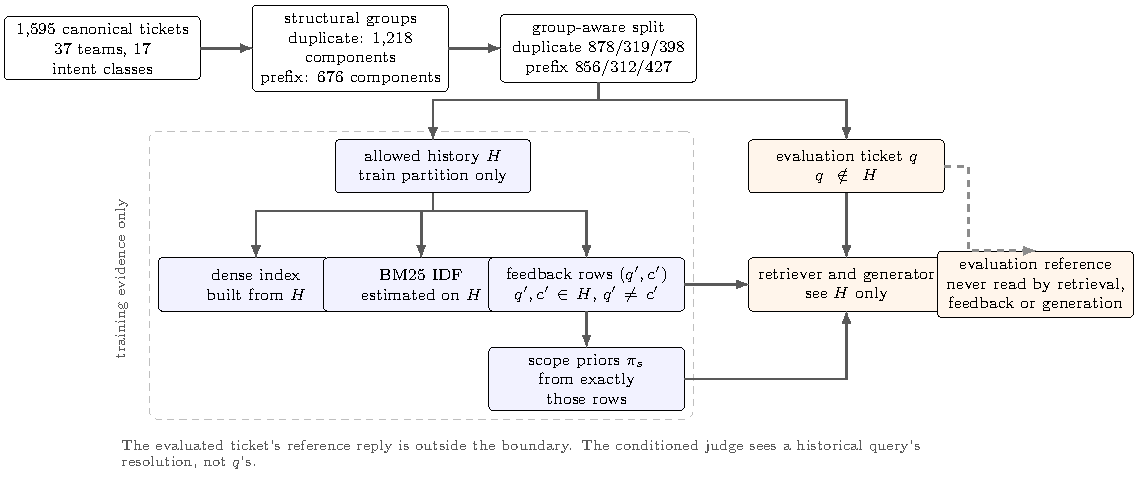
\includegraphics[width=\textwidth]{figures/fig1_regime.pdf}
\caption{Data regime and allowed history. The retriever, BM25 statistics, feedback
rows and scope priors see only the training partition $H$; the evaluation ticket's
reference reply stays outside the boundary. The conditioned judge uses a historical
query's resolution, not the evaluated ticket's reference.}
\label{fig:regime}
\end{figure*}

\subsection{Protocols and judges}
Feedback is produced twice, changing only what the judge sees. In the
\emph{conditioned} protocol the judge receives the training query, that query's
recorded resolution, and the candidate, and scores procedural equivalence on a
0--1 scale. Both the query and the candidate are historical tickets with known
resolutions, so the conditioned votes can be precomputed and used for a new query;
the judge never sees the new ticket's resolution. In the \emph{blind} protocol the
judge receives only the training query and the candidate, which is the setting
available for a new ticket at inference time. The contrast is therefore not between
an unrealizable upper bound and a deployable setting: it is a resolution-informed
judge on historical pairs versus a ticket-only judge.

Each protocol scores 878 training queries $\times$ 200 candidates $=$ 175,600
pairs at temperature 0 with a pinned model and run date. Each training query is
judged against 200 candidates, twice the evaluation pool, so that narrow scopes
retain enough documented evidence. The judge is the \texttt{gpt-5.6-luna} model at
temperature 0; the system prompt hash is \texttt{524098066b407de3}; the judging
cache dates are 12--13 September 2026. The same model is used for both protocols,
so the manipulation is what the judge sees, not which model judges.

The score distribution is zero-inflated and negative-heavy. On the allowed strict
rows, the conditioned judge assigns 62.9\,\% negative, 12.1\,\% positive and
25.0\,\% neutral scores; the blind judge assigns 57.3\,\%, 7.8\,\% and 34.9\,\%.
The full judged set contains 58.7\,\% and 48.3\,\% exact zeros. This asymmetry is a
property of the evidence, not of the lift formula, and it drives the saturation
analysis in Section~\ref{sec:repair}.

\subsection{Generation regime and provenance}
All primary runs share one generation regime: the \texttt{gpt-5.6-luna} model at
temperature 0. The system prompt hash is \texttt{524098066b407de3}; the regime
identifier is \texttt{51fd9f4b37e900bb}; and the response cache is warm. The
history-only panels were generated on 12 November 2026. Baseline answers are identical across sources of the
same panel; the freeze record in the repository verifies this ticket by ticket. A
cross-generator experiment with a different model is not pooled with this study;
the claims are within one regime. Because
hosted models can drift, all comparisons are within-regime and the artifacts record
the exact model, prompt and dates.

\subsection{Statistical protocol}
The estimand is the mean paired difference in cosine between the feedback and
baseline replies on the same tickets. We report a ticket-level paired bootstrap
interval for the mean and for the median, because the outcome is zero-inflated:
under conditioned feedback, 55.0\,\% of strict-panel and 22.6\,\% of familiar-panel
tickets have an unchanged answer. The median is exactly zero in most cells, so a
rank test has little power even when the mean interval excludes zero; we report the
Wilcoxon test as a secondary statistic and state which statistic each claim uses.
All intervals resample tickets as clusters. Paired tests are two-sided.

We fix three families before adjustment: conditioned and blind across
panels; reply similarity; and the direct conditioned-minus-blind contrast. Holm
correction is applied within each family. Exploratory analyses (scope grid, formula
ordering, expected-value selection, negative results) are labelled as such and are
not used for confirmation. The minimum detectable effect (MDE) at 80\,\% power is
reported for each primary cell; it is a sensitivity floor, not an equivalence
boundary. The eval split had already been used in the exploratory phase, so the
analyses in this article are not prospectively preregistered. We state this explicitly
rather than claiming a registration that does not exist. The analysis protocol and
the frozen artifact hashes are dated and archived.

\subsection{Data availability and ethics}
The enterprise tickets are confidential and anonymized and cannot be released.
Organizational approval was obtained for research use. The code, judge prompts,
frozen scores, run manifests, aggregate tables and figure generators are released in
the project repository; the ticket text, feedback pairs and generated answers remain
closed because they contain confidential enterprise text. The repository includes a
license file: code is released under MIT and documentation and aggregate tables
under CC BY 4.0. The expert study used anonymized tickets, stored ratings without
ticket text in any external service, and reports only aggregates. Section~\ref{sec:repro}
states exactly what a third party can rerun.


% ============================================================================
\section{Method}
\label{sec:method}

\subsection{Retrieval}
For each query the retriever returns a pool of $K=100$ tickets from the allowed
history $H$, and the generator receives the top $k=5$. The generator is called
through the Hugging Face Transformers library \cite{b29}. The primary retriever is
the frozen dense MiniLM bi-encoder \cite{b2,b28} over a FAISS index \cite{b3}; BM25
\cite{b4} and hybrid reciprocal-rank fusion \cite{b5} are used in the matched
comparison of Section~\ref{sec:repair}. All retrievers return pools of the same
size. We do not compare retriever strength under different lift configurations,
because absolute lift units are not comparable across score geometries.

\subsection{Lift}
Let $\mathrm{pos}$ and $\mathrm{neg}$ be the number of positive and negative judge
scores for candidate $c$ in scope $s$, and $n=\mathrm{pos}+\mathrm{neg}$. The
legacy Laplace lift (the formula inherited from the original pipeline) is
\begin{equation}
\begin{aligned}
p &= \frac{\mathrm{pos}+\alpha}{n+\alpha+\beta},\\
\ell_{\mathrm{L}} &= \operatorname{clamp}_{[-c,c]}\!\left(
(p-\tfrac12)\,\min\!\left(1,\tfrac{n}{2}\right)m\right),
\end{aligned}
\label{eq:legacy}
\end{equation}
with $\alpha=\beta=1$, $m=0.80$ and $c=0.20$. The empirical-Bayes lift is
\begin{equation}
\begin{aligned}
\bar p_s &= \pi_s,\qquad a=\kappa\pi_s,\\
p_{\mathrm{post}} &= \frac{\mathrm{pos}+a}{n+\kappa},\\
\ell_{\mathrm{EB}} &= \operatorname{clamp}_{[-c,c]}\!\left(
(p_{\mathrm{post}}-\pi_s)\,m\right),
\end{aligned}
\label{eq:eb}
\end{equation}
where $\pi_s$ is the mean judge score of scope $s$ over the admissible training
rows, with a global fallback when a scope has no rows. The finalist uses
$\kappa=2$. Two differences from Eq.~\ref{eq:legacy} matter: the neutral point is
the scope base rate rather than $0.5$, and the $n/2$ ramp is absent because the
centring term already attenuates sparse evidence. The legacy ramp is one of the
factors varied in the ablation, not an incidental implementation detail. A
candidate with no evidence receives $\ell=0$.

Pool-relative scaling expresses the bounded lift in retrieval-score units:
\begin{equation}
\ell'=\ell\cdot\frac{\lambda\,\sigma_{\mathrm{pool}}}{c},
\label{eq:pool}
\end{equation}
where $\sigma_{\mathrm{pool}}$ is the standard deviation of the retrieval scores in
the pool and $\lambda=1$ in the pool-scaled cells. The finalist uses absolute
scaling, so Eq.~\ref{eq:pool} is applied only in the ablation. The clamp is applied
before scaling. The parameters $\kappa$ and $\lambda$ were selected on dev over
$\{2,5,10,20,50\}$ and $\{0.25,0.5,1,2,4\}$, respectively; the per-cell values are
in the provenance table. The inherited legacy cell ($m=0.80$, $c=0.20$) is one
cell in the same sweep, not a special default.

\subsection{Scopes}
The candidate lift is routed by the recorded resolving team and the reply-derived
intent class. Global counts all training queries; Team restricts to the ticket's
team; Class to its intent class; Team$\cap$Class to the intersection, the finest
conventional scope; Backoff uses the finest scope with at least $k_{\min}=3$
observations, falling back from intersection to team to class to Global. The
finalist is Team$\cap$Class. The labels are held fixed across panels so that the
manipulated factor is the data boundary. They are recorded outcomes, not
predictions from the incoming ticket; results are therefore conditional on them,
and Section~\ref{sec:discussion} states this limitation.

\subsection{Control}
The gate is a logistic model over four feature families: intervention shape (how
many candidates the lift would promote, by how much, and the lift dispersion),
baseline quality (top-1 and top-5 scores and margin), semantic evidence
(query--candidate cosine statistics and score--lift correlations), and scope
evidence (coverage and maximum lift per scope). It is trained with grouped
cross-validation by ticket and frozen on dev. We report it as risk
control, not as a source of gain. The hindsight bound applies feedback only when it
helps on the observed outcome and therefore uses information no deployable policy
has; it bounds the headroom, not the performance of a feasible gate. The gate
numbers reported below are from the familiar-split analysis; the
strict panel supplies the always-on and hindsight-bound values, not a separately
trained gate. The expected-value analysis is exploratory and is confined to the
Appendix because its rows are two per ticket and are not independent.

\subsection{Evaluation}
The primary outcome is the per-ticket change in cosine between the generated first
reply and the recorded reference reply, averaged over the evaluation tickets. For
ticket $t$,
\begin{equation}
\Delta_t = \cos(\text{feedback reply}_t,\text{ref}_t)
           - \cos(\text{baseline reply}_t,\text{ref}_t),
\label{eq:delta}
\end{equation}
where $\text{ref}_t$ is the recorded reference reply. ROUGE-L \cite{b27} is
reported as a secondary lexical metric. The expert assessment of
Section~\ref{sec:expert} is the independent check of procedural correctness.
Because the study sample contains changed pairs only, we report the conditional
effect and the population effect, the latter as the changed share times the
conditional effect; unchanged pairs have a difference of zero by construction.

The automatic metric compares a generated reply with one recorded reply. It
rewards similarity, not resolution success, and a ticket may admit several valid
replies. BGE cosine \cite{b25} and BERTScore \cite{b26} were computed for the
familiar-split evaluation; they are not recomputed for every history-only panel because the
offline encoder is slow on CPU and the independent check in this article is the
expert assessment. The Appendix states the difference in coverage. This is a
limitation of the measurement, not a claim that cosine is a complete criterion.


% ============================================================================
\section{The Random-Split Baseline and Its Scope}
\label{sec:baseline}

The random-split baseline compares conditioned and blind feedback on the same
pipeline and candidate pools as the strict panels. Under conditioned feedback, the fine-scope reranking improves generated
first replies on eval by $+0.014$ (cosine $p=.012$); under blind feedback the same
reranking harms them by $-0.038$ ($p=.017$). The reversal is confined to the legacy
Laplace lift at Team and Team$\cap$Class scope. With the prior repaired, the blind
effect is $+0.002$ ($p=.86$), and the conditioned effect is also null: Backoff+EB
gives $+0.005$ on dev ($p=.90$) and $-0.002$ on eval ($p=.29$). No cell in this
baseline produces a confirmed calibrated gain under either protocol.

That pattern admits two readings. The first is that the judge's information decides
the sign of the effect. The second is that the evaluation allows the feedback to
profit from procedures and reply templates that the evaluation ticket shares with
the historical base, and that the apparent benefit is partly a property of the
split. The random-split baseline is consistent with both. A natural control is to
remove evaluation tickets that share a procedure or reply template with training.
The combined-hash split is one attempt at a procedure-disjoint control: it hashes
reply prefix, title and subcategory into one key. Table~\ref{tab:overlap} shows that it is not
procedure-disjoint under any component-wise definition. A ticket can share an identical full reply or a
300-character reply opening with training and still pass the filter. In the
canonical corpus, 12.8\,\% of the 390 evaluation tickets in such a split share an
identical full reply, 53.3\,\% share a reply opening, and 22.6\,\% are in the same
duplicate-union component as training. The random split is similar (14.8\,\%,
58.3\,\%, 29.1\,\%).

This article therefore reports the random-split numbers as a baseline and asks what
survives when the overlap is removed. It does not claim that the random-split sign
reversal is an artefact of the judge. It claims something narrower and more useful:
the reversal is confined to the legacy lift, and a substantial part of the measured
benefit depends on evaluation tickets that share procedures or reply templates with
history. On strict history, the blind harm disappears and the conditioned effect is
small. Section~\ref{sec:regime} reports that result; Section~\ref{sec:repair}
isolates the repair; Section~\ref{sec:expert} adds the expert check.


% ============================================================================
\section{Where the Gain Comes From}
\label{sec:regime}

Table~\ref{tab:generated} and Figure~\ref{fig:generated} report generated-answer
effects under the three data regimes with the frozen configuration (empirical Bayes,
$\kappa=2$, Team$\cap$Class, absolute scaling). Blind feedback costs $-0.0444$
$[-0.0606,-0.0285]$ when procedures overlap and becomes indistinguishable from zero
under strict disjointness ($+0.0008$ $[-0.0063,+0.0084]$, $p=.86$). The direct
protocol contrast falls from $+0.0549$ $[+0.0389,+0.0710]$ on the familiar panel to
$+0.0085$ $[+0.0016,+0.0158]$ on the strict panel. The conditioned effect is small
in every regime ($+0.0093$ to $+0.0149$); on the strict panel its cosine interval
excludes zero while the rank test is marginal ($p=.066$), ROUGE-L is not
significant, and the estimate lies below the study's 80\,\% MDE (0.0103). We
therefore describe it as a small, metric-dependent effect, not as a confirmed gain.

\Table[!btp](width=\textwidth){Generated-answer cosine difference against the
no-feedback baseline (paired, per ticket) under three data regimes and three
evidence sources. Brackets are 95\,\% ticket-level paired bootstrap intervals. The
finalist is empirical Bayes with $\kappa=2$, Team$\cap$Class scope and absolute
scaling. The direct contrast is shown in Figure~\ref{fig:generated}b. Wilcoxon $p$
for conditioned/blind: familiar .029/.00015, duplicate .002/.655, strict
.066/.856. Holm-adjusted $p$ within the primary family: familiar .117/.001,
duplicate .011/1.000, strict .197/1.000.\label{tab:generated}}{
\begin{tabular}{@{}lrrrr@{}}
\toprule
Regime & $n$ & Conditioned & Blind & Reply similarity \\
\midrule
Familiar  & 398 & $+0.0105$ $[+0.0005, +0.0212]$ & $-0.0444$ $[-0.0606, -0.0285]$ & $+0.0143$ $[+0.0047, +0.0242]$ \\
Duplicate & 398 & $+0.0149$ $[+0.0059, +0.0246]$ & $-0.0214$ $[-0.0367, -0.0073]$ & $+0.0081$ $[+0.0016, +0.0152]$ \\
Strict    & 427 & $+0.0093$ $[+0.0026, +0.0169]$ & $+0.0008$ $[-0.0063, +0.0084]$ & $+0.0026$ $[-0.0039, +0.0097]$ \\
\bottomrule
\end{tabular}}

\begin{figure*}[!t]
\centering
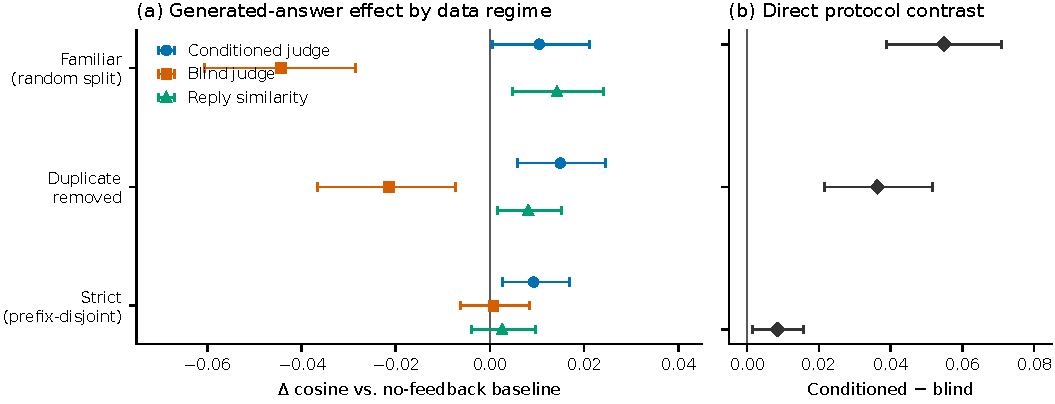
\includegraphics[width=\textwidth]{figures/fig2_generated.pdf}
\caption{Generated-answer effects by data regime. (a)~Mean $\Delta$ cosine against
the no-feedback baseline for conditioned, blind and reply-similarity evidence; bars
are 95\,\% ticket-level paired bootstrap intervals. (b)~Direct conditioned-minus-blind
contrast on the same tickets. The blind harm on the familiar panel disappears on
the strict panel, while the conditioned effect remains small.}
\label{fig:generated}
\end{figure*}

The reply-similarity baseline, which uses no LLM judge, is competitive only where
procedure overlap remains. On the familiar panel it is at least as large as the
conditioned judge ($+0.0143$ versus $+0.0105$); on the duplicate panel it is
smaller ($+0.0081$ versus $+0.0149$); on the strict panel it is $+0.0026$ with an
interval that includes zero, against $+0.0093$ for the conditioned judge. The
ordering is consistent with the overlap explanation: a simple similarity prior can
recover part of the benefit when evaluation tickets share procedures or templates
with history, but it does not replace the judge when they do not.

Three families were fixed before adjustment (conditioned and blind across panels;
reply similarity; protocol contrast) and Holm-corrected within family. Blind harm
on the familiar panel survives ($p=.0009$); the conditioned effect on the familiar
panel does not ($p=.1165$); the duplicate conditioned effect does ($p=.0106$); the
strict conditioned effect does not ($p=.1965$). The strict protocol contrast
survives ($p=.0322$) but lies below its 80\,\% MDE (0.0101). The design is not
powered to estimate an effect of that size precisely; we report it as small and
imprecisely estimated, not as evidence of absence.

At retrieval level the same pattern appears more strongly. The legacy Laplace
conditioned top-1 proxy falls from $+0.034$ on the familiar panel to $+0.002$ on
the strict panel and is significant in 0 of 5 group-aware splits; the calibrated
lift keeps a small positive point estimate ($+0.009$, 2 of 5 splits). The retrieval
proxy ranks configurations correctly but does not certify significance; the
generated intervals and the expert assessment do. This is why every claim in the
article is computed from generated answers, and the proxy is used only to select
configurations cheaply.

The interpretation is deliberately narrow. The familiar-panel conditioned gain is
not evidence that the judge recovers procedural knowledge in general; it is
evidence that a resolution-informed judge can exploit procedures and templates that
the evaluation ticket shares with history. The strict-panel conditioned interval
excludes zero, but the effect is small, metric-dependent and below the design's
MDE. The blind harm, which is the most striking result on the random split, is not
robust to the data boundary. A deployment that expects new procedures should not
budget on the familiar-panel number.


% ============================================================================
\section{Controlled Repair}
\label{sec:repair}

\subsection{One-factor ablation}
A comparison that changes scope, prior, scaling and the backoff fallback at once
cannot isolate the cause. We use a one-factor-at-a-time ablation on dev, with the
same history-only candidate pools, allowed feedback rows and selection metric for
every cell. Table~\ref{tab:ablation} reports the retrieval-level top-1 proxy; the
generated panels confirm the selected finalist, not every cell.

\Table[!btp](width=\textwidth){Controlled one-factor-at-a-time ablation on dev
(retrieval-level top-1 proxy, 319 duplicate-panel and 312 prefix-panel queries).
Every cell uses the same history-only candidate pools, allowed feedback rows and
selection metric. ``Ratio'' is $\mathrm{SD}(\text{lift})/\mathrm{SD}(\text{retrieval
score})$ within the pool. Tuned Laplace uses $m=0.60$, cap $=0.15$ on the duplicate
panel and $m=1.00$, cap $=0.05$ on the prefix panel, selected on dev. The inherited
legacy cell ($m=0.80$, cap $=0.20$) ranks 9/25 on duplicate and 23/25 on
prefix.\label{tab:ablation}}{
\begin{tabular}{@{}llrrrrr@{}}
\toprule
Configuration & Scope & Change in top-1 [95\,\% CI] & $p$ & Cap (\%) & Zero (\%) & Ratio \\
\midrule
\multicolumn{7}{@{}l}{\emph{Duplicate panel (398 tickets; 319 dev queries)}} \\
Legacy Laplace            & Team$\cap$Class & $+0.0370$ $[+0.0180, +0.0567]$ & .013 & 42.5 & 17.5 & 2.30 \\
Tuned Laplace             & Team$\cap$Class & $+0.0423$ $[+0.0248, +0.0614]$ & .001 & 42.5 & 17.5 & 1.72 \\
Laplace + pool scaling    & Team$\cap$Class & $+0.0273$ $[+0.0146, +0.0420]$ & .001 & 42.5 & 17.5 & 0.50 \\
EB $\kappa=2$, absolute   & Team$\cap$Class & $+0.0497$ $[+0.0319, +0.0688]$ & <.001 & 17.4 & 16.3 & 1.97 \\
EB $\kappa=2$ + pool       & Team$\cap$Class & $+0.0238$ $[+0.0126, +0.0368]$ & .004 & 17.4 & 16.3 & 0.45 \\
EB $\kappa=2$ + pool       & Team            & $+0.0132$ $[+0.0009, +0.0271]$ & .236 & 11.3 & 7.3 & 0.48 \\
EB $\kappa=2$ + pool       & Backoff         & $+0.0217$ $[+0.0076, +0.0370]$ & .010 & 18.9 & 0.0 & 0.54 \\
\midrule
\multicolumn{7}{@{}l}{\emph{Prefix panel (427 tickets; 312 dev queries)}} \\
Legacy Laplace            & Team$\cap$Class & $-0.0083$ $[-0.0182, +0.0004]$ & .112 & 18.1 & 68.4 & 0.95 \\
Tuned Laplace             & Team$\cap$Class & $-0.0023$ $[-0.0110, +0.0054]$ & .954 & 30.8 & 68.4 & 0.27 \\
Laplace + pool scaling    & Team$\cap$Class & $-0.0042$ $[-0.0112, +0.0013]$ & .085 & 18.1 & 68.4 & 0.21 \\
EB $\kappa=2$, absolute   & Team$\cap$Class & $-0.0008$ $[-0.0078, +0.0054]$ & .816 & 7.9 & 68.0 & 0.75 \\
EB $\kappa=2$ + pool       & Team$\cap$Class & $-0.0002$ $[-0.0033, +0.0033]$ & .358 & 7.9 & 68.0 & 0.17 \\
EB $\kappa=2$ + pool       & Team            & $-0.0002$ $[-0.0078, +0.0066]$ & .968 & 6.7 & 19.2 & 0.26 \\
EB $\kappa=2$ + pool       & Backoff         & $-0.0052$ $[-0.0131, +0.0020]$ & .845 & 30.5 & 0.1 & 0.61 \\
\bottomrule
\end{tabular}}

The inherited legacy cell is not the best Laplace configuration. It ranks 9th of
25 on the duplicate panel and 23rd of 25 on the strict panel. Tuning moves the
duplicate proxy from $+0.0370$ to $+0.0423$ and the strict proxy from $-0.0083$ to
$-0.0023$. Pool-relative scaling alone reduces the lift/score standard-deviation
ratio from 2.30 to 0.50 on duplicate and from 0.95 to 0.21 on strict. Scale is
therefore a major cause of the baseline behaviour, and the prior alone is not. On
the duplicate panel the empirical-Bayes absolute cell reaches $+0.0497$, but the
scope change to Team costs about half of that ($+0.0238$ to $+0.0132$) and the
backoff does not recover it ($+0.0217$). On the strict panel every cell is at or
below zero. This is why we describe the repair as harm removal, not as
a gain mechanism.

\subsection{Matched retrievers}
Comparing retrievers under different lift configurations confounds retriever
strength with calibration. We repeat the comparison with one feedback
configuration (empirical Bayes, $\kappa=2$, pool-relative scaling
$\lambda=1$, Team$\cap$Class) across dense MiniLM, BM25 and hybrid RRF.
Table~\ref{tab:matched} and Figure~\ref{fig:matched} report the result.

\Table[!btp](width=\textwidth){Feedback gain under one configuration (EB
$\kappa=2$, pool-relative scaling $\lambda=1$, Team$\cap$Class) across retrieval
families. Brackets are 95\,\% bootstrap intervals. Absolute scaling is omitted
because lift units are not comparable across retrievers.\label{tab:matched}}{
\begin{tabular}{@{}lrrrr@{}}
\toprule
Retriever & Familiar change & $p$ & Strict change & $p$ \\
\midrule
Dense MiniLM & $+0.0334$ $[+0.0202, +0.0475]$ & $<.001$ & $+0.0078$ $[+0.0030, +0.0137]$ & .131 \\
BM25         & $+0.0641$ $[+0.0466, +0.0821]$ & $<.001$ & $+0.0088$ $[+0.0021, +0.0167]$ & .054 \\
Hybrid RRF   & $+0.0595$ $[+0.0426, +0.0771]$ & $<.001$ & $+0.0063$ $[+0.0006, +0.0121]$ & .293 \\
\bottomrule
\end{tabular}}

\begin{figure*}[!t]
\centering
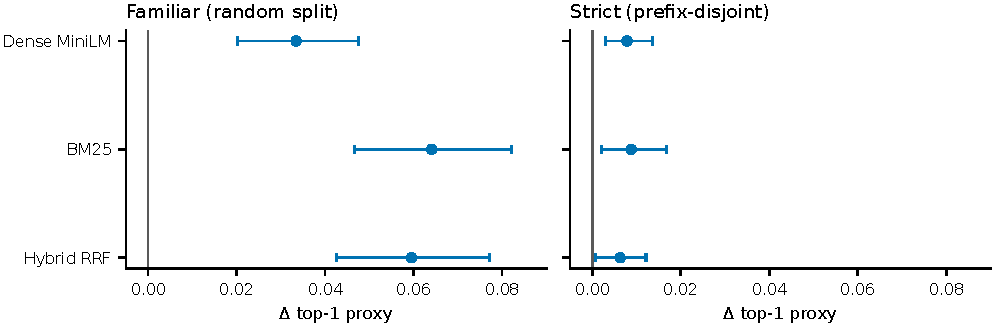
\includegraphics[width=\textwidth]{figures/fig3_matched.pdf}
\caption{Feedback gain under one configuration (EB $\kappa=2$, pool-relative
scaling $\lambda=1$) for dense MiniLM, BM25 and hybrid RRF. Bars are 95\,\%
bootstrap intervals. The claim that stronger retrieval reduces the benefit is not
supported once the lift configuration is held fixed.}
\label{fig:matched}
\end{figure*}

The feedback gain is similar across retrieval families: on the familiar panel
$+0.0334$, $+0.0641$ and $+0.0595$; on the strict panel $+0.0078$, $+0.0088$ and
$+0.0063$. The conclusion that stronger retrieval reduces the benefit is a scaling artefact:
absolute lift units are cosine units and are not meaningful on BM25 scores. We
withdraw that conclusion. This article does not claim that retriever choice is
irrelevant; it claims that the confounded comparison could not separate retriever
strength from lift scale.

\subsection{Mechanism}
The blind failure is arithmetic before it is statistical. The judge is
negative-heavy: on the allowed strict rows, 62.9\,\% of conditioned and 57.3\,\% of
blind scores are negative, against 12.1\,\% and 7.8\,\% positive. With zero
positive and two negative votes, Eq.~\ref{eq:legacy} gives $p=0.25$ and
$\ell=(0.25-0.5)\cdot1\cdot0.8=-0.20$, exactly the negative cap. More negatives
change nothing: two negative votes and twenty receive the same penalty. The
formula is antisymmetric, and two positive votes with no negatives reach the
positive cap in exactly the same way. The observed asymmetry is therefore a
property of the evidence distribution, not of the prior: the judge supplies many
more negatives than positives.

Figure~\ref{fig:saturation} measures the consequence. Under the legacy lift,
13.2\,\% of conditioned candidates with two votes sit at the negative cap and
0.15\,\% at the positive cap; for blind, the shares are 9.1\,\% and 0\,\%. At five
votes the negative-cap share is 15.6\,\% (conditioned) and 7.0\,\% (blind), while
the positive-cap share is 0\,\%. The cap turns the bonus into a near-constant
penalty for a large part of the pool. In the strict dev ablation, the
empirical-Bayes negative-cap share is 7.9\,\% and the positive cap remains
negligible.

\begin{figure*}[!t]
\centering
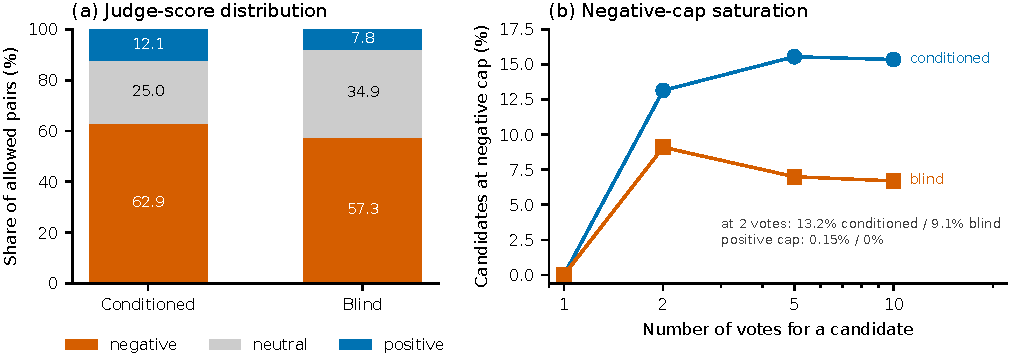
\includegraphics[width=\textwidth]{figures/fig4_saturation.pdf}
\caption{Lift saturation. (a)~Judge-score distribution on the allowed strict rows:
negative, neutral and positive shares for conditioned and blind feedback. (b)~Share
of candidates at the negative cap as a function of the number of votes. The
negative-cap mass is a property of the evidence distribution interacting with the
legacy ramp; the positive cap is negligible in both protocols.}
\label{fig:saturation}
\end{figure*}

\subsection{Control as risk control}
The gate is not a source of gain. It pays when the uncalibrated prior concentrates
harm and becomes mostly redundant once the prior is repaired. On the strict blind
panel, always-on is $+0.0008$ and the hindsight upper bound is $+0.0190$, so the
maximum headroom is 0.0182. On the familiar blind panel, always-on is $-0.0444$ and
the hindsight bound is $+0.0258$, headroom 0.0701. A feasible gate can capture only a
fraction of that headroom, and we do not claim that it recovers the ceiling. In the
familiar-split analysis, the gate was trained once across signals and protocols with
grouped cross-validation by ticket; its dev out-of-fold AUC was 0.699
$[0.676,0.721]$, and eval AUC ranged from 0.56 to 0.74. The feature-family
ablation showed that intervention shape carried the signal (AUC 0.681), while
baseline quality (0.553), semantic cosine (0.548) and scope evidence (0.548) added
little. This is consistent with the mechanism: the gate
predicts pool reshaping, not similarity.

The exploratory expected-value analysis pooled conditioned and blind
rows, which are two per ticket and not independent. We do not use that analysis for
a main claim. It is reported in the Appendix as exploratory, with the
non-independence caveat, and it is not used to compare a protocol a deployed system
cannot run with one it can.


% ============================================================================
\section{Expert Assessment of Procedural Correctness}
\label{sec:expert}

The automatic metric compares a generated reply with one recorded reply. To check
whether that similarity tracks procedural correctness, we asked support engineers
to rate a blinded sample. The sample contains 105 changed pairs, 35 in each of
three arms: familiar procedures with blind feedback, new procedures with blind
feedback, and new procedures with conditioned feedback. A pair is eligible only if
the feedback answer differs from the baseline answer; unchanged pairs would add no
information. The sample is stratified by resolving team, A/B order is randomized
and balanced within each arm, and no ticket appears in two arms. The study is a
validity check, not a confirmatory trial: the arms contain only 2--7 discordant
pairs, and one expert has completed the sample while the second is in progress.

For each reply the expert marked correct, partially correct, incorrect or cannot
judge, flagged a wrong or unsafe step and a missing required step, and then chose
the better reply, with equal, both incorrect and cannot judge as explicit options.
Strict correctness counts only ``correct''; lenient correctness also counts
``partially correct''. Intervals are paired bootstrap intervals over tickets;
p-values are exact McNemar tests on discordant pairs. Table~\ref{tab:expert} and
Figure~\ref{fig:expert} report the first expert's results.

\Table[!btp](width=\textwidth){Blinded expert assessment of procedural correctness
(E1; 105 items, 35 per arm). Strict correctness counts only ``correct''. Intervals
are paired bootstrap intervals over tickets; $p$ is the exact McNemar test on
discordant pairs. Four items were cannot-judge and are excluded from the paired
analysis. Discordant pairs: 7, 3 and 2. Across all 105 items: 42 equal, 32 both
incorrect, 2 cannot judge. On the familiar arm the feedback replies are 173
characters longer; the expert preference tracks length (Spearman $+0.63$) and is
zero among length-matched pairs. The second expert is in progress; agreement is not
yet reported.\label{tab:expert}}{
\begin{tabular}{@{}lrrrrr@{}}
\toprule
Arm & $n$ & Baseline & Feedback & Difference [95\,\% CI] & $p$ \\
\midrule
Familiar, blind       & 34 & 0.647 & 0.794 & $+0.147$ $[0.000, +0.294]$ & .25 \\
Strict, blind         & 33 & 0.545 & 0.515 & $-0.030$ $[-0.121, +0.061]$ & 1.00 \\
Strict, conditioned   & 34 & 0.559 & 0.559 & $0.000$ $[-0.088, +0.088]$ & 1.00 \\
\bottomrule
\end{tabular}}

\begin{figure*}[!t]
\centering
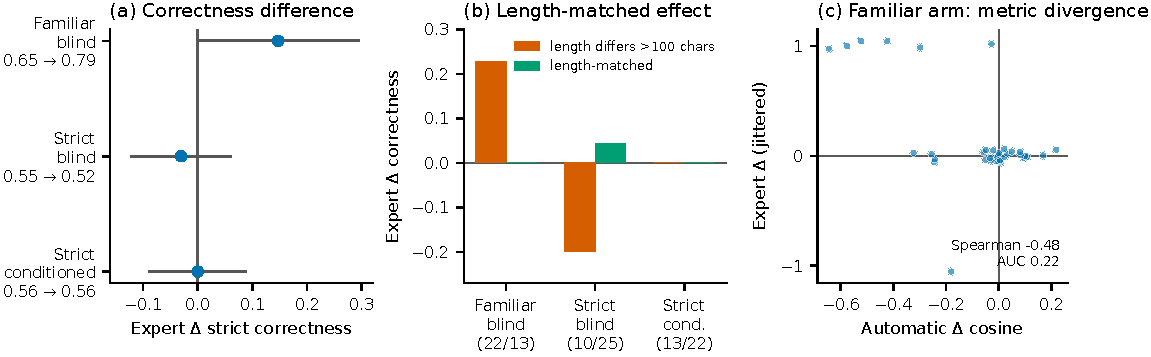
\includegraphics[width=\textwidth]{figures/fig5_expert.pdf}
\caption{Expert assessment (E1). (a)~Strict-correctness difference between feedback
and baseline with 95\,\% paired bootstrap intervals; the labels show the baseline
and feedback rates. (b)~Effect among length-matched pairs versus pairs whose lengths
differ by more than 100 characters; sample sizes are unmatched/matched. (c)~Automatic
cosine difference versus expert difference on the familiar arm; the two measures
point in opposite directions.}
\label{fig:expert}
\end{figure*}

Three results matter. First, on the strict panels the expert does not confirm
benefit or harm: both intervals include zero and the point estimates are within $\pm0.03$,
matching the small automatic effects there. Second, the familiar arm shows a raw
$+0.147$, but the feedback replies are 173 characters longer and the expert
preference tracks that difference (Spearman $+0.63$); among pairs whose lengths
differ by at most 100 characters the effect is exactly zero (n=13). The apparent
benefit on familiar procedures is a preference for longer, more detailed replies,
not a demonstrated procedural improvement. Third, the expert and the cosine metric
point in opposite directions on that arm (expert $+0.147$, automatic $-0.088$;
Spearman $-0.48$, AUC 0.22). Neither measure is a clean criterion: cosine rewards
similarity to one recorded reply, and the expert is sensitive to answer length.

The preference data show why the per-reply correctness rating was necessary.
Across the sample, 42 items were rated equal and 32 both incorrect; a raw A/B
preference alone would have hidden a third of the sample as ``both wrong''. The
unsafe-step and missing-step flags were rare (5.7--8.6\,\% for unsafe steps,
0--2.9\,\% for missing steps), so we report them descriptively and do not treat
them as evidence of a safety difference. With 2--7 discordant pairs per arm, the
study can detect only an almost perfectly consistent advantage; the intervals, not
the p-values, are the result. We do not claim that the expert confirms either the
automatic harm or the automatic benefit.

The second expert will be analysed with the same fixed pipeline. When the sample is
complete we will add percent agreement, Cohen's $\kappa$ with a bootstrap interval,
weighted $\kappa$ for the ordinal correctness rating, PABAK/AC1 as a
prevalence-robust sensitivity, and a combined per-item estimate on the common items.
The analysis supports partial overlap: if the second expert does not finish all 105
items, the agreement and combined estimate use the items both experts rated, and
the coverage is reported explicitly. The sample, answers, A/B assignment and
analysis plan are frozen; no item is added or removed after the first rating.


% ============================================================================
\section{Validation}
\label{sec:validation}

\subsection{Secondary metric and seeds}
ROUGE-L agrees in sign with cosine on all three panels, but on the strict
conditioned panel its interval includes zero ($+0.0034$ $[-0.0036,+0.0105]$,
$p=.47$), and on the strict blind panel it is $+0.0020$ $[-0.0049,+0.0093]$
($p=.53$). We report it as a secondary metric, not as
confirmation. The strict conditioned cosine interval excludes zero, but the lexical
metric does not; this is one reason we call the effect metric-dependent.

Five group-aware splits were generated for each structural rule. On the strict
panel the legacy Laplace blind proxy is negative and significant in 4 of 5 splits,
while the calibrated blind proxy is significant in 0 of 5; the calibrated point
estimate remains slightly negative ($-0.0030$ to $-0.0005$). For conditioned
feedback, the legacy Laplace proxy is significant in 0 of 5 strict splits, while
the calibrated lift has a small positive point estimate in 2 of 5. The generated
panels use seed 42; the other seeds test the retrieval-level conclusion and are not
a second set of generated answers. The direction of the blind result is stable
across seeds; the conditioned result is small enough that seed variation matters.

\subsection{Power and multiplicity}
The minimum detectable effect at 80\,\% power is 0.0103 for the strict conditioned
cosine effect and 0.0101 for the strict protocol contrast. The observed values are
0.0093 and 0.0085, so the design is not powered to estimate effects of that size
precisely. We describe them as small and imprecise, not as evidence of absence. An
equivalence claim would require a pre-specified margin and a corresponding test; we
do not make one. Three families were fixed before adjustment (conditioned and blind
across panels; reply similarity; protocol contrast) and Holm-corrected within
family. The strict conditioned effect does not survive ($p=.1965$); the strict
protocol contrast does ($p=.0322$) but lies below its MDE. The familiar blind harm
survives ($p=.0009$), which is the one primary result that is both significant and
above its MDE.

\subsection{Cost}
Table~\ref{tab:cost} reports end-to-end generation cost from the frozen runs.
Generation takes 0.48--0.87 seconds per request on CPU, with two requests per ticket
for baseline and feedback; a panel of 398--427 tickets takes 356--617 seconds. The
calibrated lift adds no model call at inference; its cost is the offline feedback
construction. Feedback-database preparation is a separate one-off cost and is not
included. The cost is compatible with batch first-reply generation; it is not a
real-time guarantee.

\Table[!btp](width=\textwidth){End-to-end generation cost from the frozen runs
(CPU, model loading and metric computation included). Each ticket uses two
requests, baseline and feedback. Feedback-database preparation is a separate
one-off cost.\label{tab:cost}}{
\begin{tabular}{@{}lrrrr@{}}
\toprule
Regime / source & Queries & Requests & Seconds & s/request \\
\midrule
Familiar / conditioned    & 398 & 709 & 616.6 & 0.87 \\
Familiar / blind          & 398 & 749 & 363.0 & 0.48 \\
Familiar / reply sim.     & 398 & 740 & 357.2 & 0.48 \\
Duplicate / conditioned   & 398 & 671 & 564.0 & 0.84 \\
Duplicate / blind         & 398 & 696 & 355.5 & 0.51 \\
Duplicate / reply sim.    & 398 & 686 & 355.5 & 0.52 \\
Strict / conditioned      & 427 & 625 & 532.0 & 0.85 \\
Strict / blind            & 427 & 636 & 426.0 & 0.67 \\
Strict / reply sim.       & 427 & 611 & 436.5 & 0.71 \\
\bottomrule
\end{tabular}}

\subsection{What is not validated}
This article does not have an external corpus, a second organization, real user
feedback, or a completed second expert. BGE and BERTScore are not recomputed for
every history-only panel; the independent check is the expert assessment, and it is one
rater at the time of writing. The automatic metric compares to one recorded reply,
and the routing labels are recorded outcomes rather than predictions. Hosted models
can drift; the generation regime and hashes are pinned, but bit-level
reproducibility is not claimed. These are limits on generalization and measurement,
not implementation details, and Section~\ref{sec:discussion} states them as such.


% ============================================================================
\section{Discussion and Limitations}
\label{sec:discussion}

\subsection{What the result changes}
Three practical consequences follow. First, a feedback gain measured on a random
split should be re-measured after removing near-duplicate procedures and reply
templates; otherwise the number describes the data regime as much as the method.
The familiar-panel blind effect is $-0.0444$; on strict history it is $+0.0008$.
A team that budgets on the first number will overstate both the risk and the
opportunity. Second, tuning the legacy baseline matters. The inherited Laplace cell
ranks 23rd of 25 on the strict panel; an untuned lift is not a fair comparator, and
a tuned one still does not produce a confirmed gain on strict history. Third,
similarity to a single recorded reply is not procedural correctness. The expert and
the cosine metric diverge on the familiar arm, and the expert's preference is
itself sensitive to answer length. Evaluation protocols should state the evidence
set, keep the prior aligned with it, and add an expert check with length control.

The result also changes the interpretation of the random-split sign reversal. The
reversal is real for the legacy Laplace lift on the familiar split: the same
reranking helps under a resolution-informed judge and harms under a ticket-only
judge. But the blind harm is not robust to the data boundary, and the conditioned
gain is small on strict history. The accurate summary is narrower than ``the judge
decides the sign'': an uncalibrated popularity lift can help under one judge and
hurt under another on overlapping data, while a calibrated lift removes the harm
without a confirmed gain on new procedures.

\subsection{What we do not claim}
We do not claim a deployable improvement. The calibrated blind gain is not
significant and lies below its run-specific detection threshold; the conditioned
protocol is a resolution-informed upper bound for historical pairs, not a claim that
a new ticket's resolution is available. The feedback is simulated by an LLM judge,
not collected from users. The findings come from one organizational corpus and one
language; external validity is untested. The primary quality metric is similarity
to one recorded reply, not verified resolution success, and per-ticket agreement
between metrics and the expert is limited even when aggregate directions agree.
The alternative-retriever comparison is matched on the feedback configuration but
still uses one corpus and one generator. The secondary analyses (scope grid, formula
ordering, expected-value selection, negative results) are exploratory and are not
used for confirmation. We do not claim that calibration and control are generally
substitutable; we claim that in the tested configurations the gate adds little once
the prior is calibrated, and that it pays mainly where always-on is harmful.

\subsection{Limitations}
The corpus is a single enterprise in a single language. The expert study uses 105
changed pairs, 35 per arm; with 2--7 discordant pairs per arm it can detect only
large differences, and one expert is not a population sample. The second expert is
in progress; until the sample is complete, no inter-rater agreement is reported.
Procedural correctness is not ticket resolution, and the automatic metric compares
to one recorded reply. Feedback is simulated by an LLM judge, not collected from
users. Routing labels are the recorded resolving team and the reply-derived intent
class, so the results are label-conditional; a production system would need a
predictor or a human routing step. Hosted-model drift is bounded by a frozen
generation regime and hashed artifacts, not eliminated. BGE and BERTScore are not
recomputed for every history-only panel; the independent check is the expert
assessment.

\subsection{Threats to validity}
\textbf{Construct validity.} Cosine similarity to a single reference reply is a
proxy for usefulness, not resolution success; a ticket may admit several valid
replies. The expert assessment reduces this threat but does not eliminate it: the
expert judges procedural correctness from the ticket and the two replies, and the
rubric is sensitive to answer length. The feedback judge is resolution-informed on
historical pairs, so it measures procedural equivalence to a recorded resolution,
not the usefulness of a reply to a new user.

\textbf{Internal validity.} The data regimes share the corpus and the generation
regime, which strengthens within-study contrasts but limits causal isolation. The
strict panel changes the data boundary and the candidate pool together; the
ablation isolates the lift factors, not every possible confound. The split audit
shows that the combined-hash split was not disjoint, but it does not prove
that every remaining difference between panels is due to overlap. The matched
retriever comparison holds the feedback configuration fixed, but it still uses one
generator and one corpus.

\textbf{External validity.} The corpus is one enterprise in one language; absolute
effect sizes should not be transferred without re-validation. The saturation
diagnostic is cheap and portable, and we release it so that others can compute it
on their own feedback sources. The practical recipe in Section~\ref{sec:discussion}
is a set of hypotheses to test, not a general law.

\textbf{Statistical validity.} The MDE is run-specific and states the effect sizes
the study could reliably detect; it is not an equivalence boundary. The strict
conditioned effect and the strict protocol contrast are below their MDEs, so we
describe them as small and imprecise. The familiar blind harm is above its MDE and
survives Holm correction; the strict conditioned effect does not survive Holm. The
two-blind-run agreement at four decimals on the familiar split is a coincidence
of aggregation: the runs differ per ticket (mean absolute difference 0.0671,
median 0.0337, 11.8\,\% identical deltas, $r=.799$), and both inherit the saturated
prior.

\subsection{Practical implications}
This article suggests a short checklist for teams that use feedback reranking.
(1)~\emph{Measure overlap first}: report the share of evaluation tickets that share
a full reply, a reply opening, or a title+subcategory signature with training.
(2)~\emph{Align the prior with the allowed evidence}: estimate the scope base rate
from exactly the feedback rows that are admissible, and state the estimator.
(3)~\emph{Tune the baseline}: compare against a tuned Laplace cell under a matched
selection budget, not only against the inherited parameters. (4)~\emph{Add a reply-similarity baseline that uses no LLM judge}: if it matches the LLM judge, the judge may be buying
overlap rather than procedure. (5)~\emph{Check a sample with experts}: use blinded
A/B order, per-reply correctness, explicit ties and both-incorrect options, and a
length control. (6)~\emph{Treat a gate as risk control}: it pays where always-on is
harmful, not as a general source of gain. These are hypotheses to test on other
corpora, not a guarantee.


% ============================================================================
\section{Conclusion}
\label{sec:conclusion}

The same reranking can look helpful or harmful depending on what the judge knows,
but the larger determinant in our data is whether evaluation tickets share
procedures or reply templates with the historical base. When they do not, the blind
harm disappears, the calibrated gain is small and metric-dependent, and a
reply-similarity prior that uses no LLM judge no longer matches the LLM judge. The
expert assessment does not confirm harm or benefit on new procedures and shows that
the familiar-procedure preference is explained by reply length. We conclude that feedback reranking gains
reported on overlapping splits are partly borrowed from procedure overlap, that
calibration removes harm without a confirmed gain, and that similarity to one
recorded reply is not procedural correctness. The practical recipe is a set of
hypotheses to test in other corpora, not a general law. The open questions are how
the findings transfer to a second organization, to real user feedback, and to
expert ratings from a larger and fully overlapped sample; the released artifacts
and the frozen protocol make those replications directly comparable.


\appendix
\section{Supplementary Analyses}
\label{sec:appendix}

\subsection{Seed robustness}
Table~\ref{tab:seed} reports the strict-panel retrieval proxy across the five
group-aware splits for the three configurations that matter for the argument: the
legacy Laplace lift, empirical Bayes with absolute scaling, and empirical Bayes with
pool-relative scaling. The blind harm is significant in 4 of 5 legacy splits and in
0 of 5 calibrated splits; the conditioned calibrated lift is significant in 2 of 5.
The table is a robustness check, not a second generated panel.

\Table[!btp](width=\textwidth){Strict-panel retrieval-level robustness across five
group-aware splits (seed 42 plus four alternatives). Entries are mean top-1 proxy
differences, with the range across seeds and the number of seeds significant at
$p<.05$.\label{tab:seed}}{
\begin{tabular}{@{}llrrr@{}}
\toprule
Protocol & Configuration & Mean change & Range & Significant \\
\midrule
Blind & Legacy Laplace & $-0.0084$ & $[-0.0116, -0.0046]$ & 4/5 \\
Blind & EB $\kappa=2$, absolute & $-0.0030$ & $[-0.0069, -0.0001]$ & 1/5 \\
Blind & EB $\kappa=2$, pool & $-0.0005$ & $[-0.0024, +0.0025]$ & 0/5 \\
Conditioned & Legacy Laplace & $+0.0023$ & $[-0.0057, +0.0055]$ & 0/5 \\
Conditioned & EB $\kappa=2$, absolute & $+0.0088$ & $[+0.0058, +0.0105]$ & 2/5 \\
Conditioned & EB $\kappa=2$, pool & $+0.0055$ & $[+0.0029, +0.0078]$ & 1/5 \\
\bottomrule
\end{tabular}}

\subsection{Two concrete cases}
The running ticket illustrates the blind failure. Ticket R-377 (``Connect to Client
SW'') mentions a product name shared by a network appliance and a locally installed
application. The baseline ranks a network-access reply first: the words match, the
procedure does not. Under blind feedback, the correct software candidate carries
sparse evidence and is pinned near the negative cap, while the wrong but popular
network candidate keeps a small penalty; the blind reranking leaves the wrong
candidate on top and the generated reply keeps the network procedure
($\Delta=-0.03$). Under conditioned feedback, the judge that knows the resolution
votes for the software candidate, the lift promotes it, and the generated reply
moves to the software procedure ($\Delta=+0.540$). The contrast is the mechanism in
one instance, not a representative effect size.

A second case illustrates a calibrated-neutral outcome. Ticket R-1130 has one
intersection-scope observation (0.8 positive, 0.2 negative). The calibrated lift is
bounded, the top-1 candidate is unchanged, and the generated reply is identical to
the baseline ($\Delta=0$). Calibration does not force a change when the evidence
does not justify one; this is the intended behaviour, and it is why the calibrated
distribution has a large mass at zero rather than a uniform positive shift.

\subsection{Reproduction and artifacts}
\label{sec:repro}
A third party can rerun three levels. (i) From the public repository, without
confidential data: the aggregate tables and figures, the human-evaluation analysis
from aggregate or raw ratings on premises, the unit tests, and the data-protocol
validation on synthetic data. (ii) With the confidential corpus on premises: the
full pipeline, retrieval panels and generated panels with an API key. (iii) With new
API calls: generation and judging can be repeated, but hosted models may drift; the
generation regime and hashes are pinned rather than claiming bit-level
reproducibility. The generator and judge are the \texttt{gpt-5.6-luna} model at
temperature 0; the full API identifier is \mbox{\texttt{openai/gpt-5.6-luna}}.
The generation regime is \texttt{51fd9f4b37e900bb}; the system
prompt hash is \texttt{524098066b407de3}. The finalist uses $\kappa=2$, absolute
scaling, Team$\cap$Class scope, top-5 context, and a 100-candidate pool. The
scope base rate $\pi_s$ is the mean judge score per scope over the allowed training
rows, with a global fallback. The repository includes the frozen run manifest, the
table and figure generators, and a license file (MIT for code; CC BY 4.0 for
documentation and aggregate tables; confidential data not released).

\subsection{Exploratory analyses}
The Appendix also records the analyses that are not used for confirmation. The
scope grid shows that broad pooling harms under both protocols while fine scopes
help; the formula ordering places empirical Bayes above tanh, Laplace and Bayesian
LCB offline; the expected-value analysis uses gradient boosting \cite{b23} and a
Ridge linear control \cite{b24}, pools conditioned and blind rows, and is therefore
exploratory; and the negative-results map records a semantic relevance
filter, a learned scope blend, a hybrid-transfer failure under a different lift
configuration, and sign-based multi-action selection. These results map the
boundaries of the method and are reported with their mechanisms in the repository.
This article does not use them to support the main claim.


\begin{thebibliography}{43}

\bibitem{b1} P. Lewis \emph{et al.}, ``Retrieval-augmented generation for knowledge-intensive NLP tasks,'' in \emph{Proc. Adv. Neural Inf. Process. Syst. (NeurIPS)}, vol. 33, 2020, pp. 9459--9474.

\bibitem{b2} N. Reimers and I. Gurevych, ``Sentence-BERT: Sentence embeddings using Siamese BERT-networks,'' in \emph{Proc. Conf. Empirical Methods Natural Lang. Process. (EMNLP-IJCNLP)}, 2019, pp. 3982--3992.

\bibitem{b3} J. Johnson, M. Douze, and J. H\'egou, ``Billion-scale similarity search with GPUs,'' \emph{IEEE Trans. Big Data}, vol. 7, no. 3, pp. 535--547, 2021.

\bibitem{b4} S. Robertson and H. Zaragoza, ``The probabilistic relevance framework: BM25 and beyond,'' \emph{Found. Trends Inf. Retr.}, vol. 3, no. 4, pp. 333--389, 2009.

\bibitem{b5} G. V. Cormack, C. L. A. Clarke, and S. Buettcher, ``Reciprocal rank fusion outperforms Condorcet and individual rank learning methods,'' in \emph{Proc. ACM SIGIR}, 2009, pp. 758--759.

\bibitem{b6} R. Nogueira and K. Cho, ``Passage re-ranking with BERT,'' \emph{arXiv:1901.04085}, 2019.

\bibitem{b7} V. Karpukhin \emph{et al.}, ``Dense passage retrieval for open-domain question answering,'' in \emph{Proc. Conf. Empirical Methods Natural Lang. Process. (EMNLP)}, 2020, pp. 6769--6781.

\bibitem{b8} J. J. Rocchio, ``Relevance feedback in information retrieval,'' in \emph{The SMART Retrieval System: Experiments in Automatic Document Processing}, 1971, pp. 313--323.

\bibitem{b9} V. Lavrenko and W. B. Croft, ``Relevance-based language models,'' in \emph{Proc. ACM SIGIR}, 2001, pp. 120--127.

\bibitem{b10} H. Abdollahpouri, R. Burke, and B. Mobasher, ``Managing popularity bias in recommender systems with personalized re-ranking,'' in \emph{Proc. Int. Florida Artif. Intell. Res. Soc. Conf. (FLAIRS)}, 2019, pp. 413--418.

\bibitem{b11} L. Zheng \emph{et al.}, ``Judging LLM-as-a-judge with MT-Bench and Chatbot Arena,'' in \emph{Proc. Adv. Neural Inf. Process. Syst. (NeurIPS)}, 2023.

\bibitem{b12} Y. Liu \emph{et al.}, ``G-Eval: NLG evaluation using GPT-4 with better human alignment,'' in \emph{Proc. Conf. Empirical Methods Natural Lang. Process. (EMNLP)}, 2023, pp. 2511--2522.

\bibitem{b13} P. Wang \emph{et al.}, ``Large language models are not fair evaluators,'' in \emph{Proc. Annu. Meeting Assoc. Comput. Linguistics (ACL)}, 2024, pp. 9440--9450.

\bibitem{b14} A. Panickssery, S. R. Bowman, and S. Feng, ``LLM evaluators recognize and favor their own generations,'' in \emph{Proc. Adv. Neural Inf. Process. Syst. (NeurIPS)}, 2024.

\bibitem{b15} J. Platt, ``Probabilistic outputs for support vector machines and comparisons to regularized likelihood methods,'' in \emph{Advances in Large Margin Classifiers}, 1999, pp. 61--74.

\bibitem{b16} B. Zadrozny and C. Elkan, ``Transforming classifier scores into accurate multiclass probability estimates,'' in \emph{Proc. ACM SIGKDD}, 2002, pp. 694--699.

\bibitem{b17} A. Niculescu-Mizil and R. Caruana, ``Predicting good probabilities with supervised learning,'' in \emph{Proc. Int. Conf. Mach. Learn. (ICML)}, 2005, pp. 625--632.

\bibitem{b18} H. Robbins, ``An empirical Bayes approach to statistics,'' in \emph{Proc. 3rd Berkeley Symp. Math. Statist. Probab.}, 1956, pp. 157--163.

\bibitem{b19} I. J. Good, \emph{The Estimation of Probabilities: An Essay on Modern Bayesian Methods}. Cambridge, MA, USA: MIT Press, 1965.

\bibitem{b20} C. K. Chow, ``On optimum recognition error and reject tradeoff,'' \emph{IEEE Trans. Inf. Theory}, vol. 16, no. 1, pp. 41--46, 1970.

\bibitem{b21} Y. Geifman and R. El-Yaniv, ``Selective classification for deep neural networks,'' in \emph{Proc. Adv. Neural Inf. Process. Syst. (NeurIPS)}, 2017, pp. 4878--4887.

\bibitem{b22} C. Elkan, ``The foundations of cost-sensitive learning,'' in \emph{Proc. Int. Joint Conf. Artif. Intell. (IJCAI)}, 2001, pp. 973--978.

\bibitem{b23} G. Ke \emph{et al.}, ``LightGBM: A highly efficient gradient boosting decision tree,'' in \emph{Proc. Adv. Neural Inf. Process. Syst. (NeurIPS)}, 2017, pp. 3146--3154.

\bibitem{b24} F. Pedregosa \emph{et al.}, ``Scikit-learn: Machine learning in Python,'' \emph{J. Mach. Learn. Res.}, vol. 12, pp. 2825--2830, 2011.

\bibitem{b25} S. Xiao, Z. Liu, P. Zhang, and N. Muennighoff, ``C-Pack: Packed resources for general Chinese embeddings,'' in \emph{Proc. ACM SIGIR}, 2024, pp. 641--649.

\bibitem{b26} T. Zhang, V. Kishore, F. Wu, K. Q. Weinberger, and Y. Artzi, ``BERTScore: Evaluating text generation with BERT,'' in \emph{Proc. Int. Conf. Learn. Represent. (ICLR)}, 2020.

\bibitem{b27} C.-Y. Lin, ``ROUGE: A package for automatic evaluation of summaries,'' in \emph{Proc. ACL Workshop Text Summarization Branches Out}, 2004, pp. 74--81.

\bibitem{b28} J. Devlin, M.-W. Chang, K. Lee, and K. Toutanova, ``BERT: Pre-training of deep bidirectional transformers for language understanding,'' in \emph{Proc. Conf. North Amer. Chapter Assoc. Comput. Linguistics (NAACL)}, 2019, pp. 4171--4186.

\bibitem{b29} T. Wolf \emph{et al.}, ``Transformers: State-of-the-art natural language processing,'' in \emph{Proc. Conf. Empirical Methods Natural Lang. Process. (EMNLP): System Demonstrations}, 2020, pp. 38--45.

\bibitem{b31} D. Jer\v{s}ek, K. Kenda, R. Klan\v{c}i\v{c}, and M. Frattini, ``Automated first-reply generation for IT support tickets using retrieval-augmented generation and multi-modal response synthesis,'' in \emph{Proc. Information Society (SIKDD)}, Ljubljana, Slovenia, 2025.

\bibitem{b32} D. Jer\v{s}ek, B. Ka\v{z}i\v{c}, and K. Kenda, ``Exploring feedback-aware retrieval for IT support first-reply generation,'' in \emph{Proc. Information Society (SIKDD)}, Ljubljana, Slovenia, 2026.

\bibitem{b33} DeepSeek-AI, ``DeepSeek-V4: Towards highly efficient million-token context intelligence,'' \emph{arXiv:2606.19348}, 2026.

\bibitem{b34} T. Joachims, L. Granka, B. Pan, H. Hembrooke, and G. Gay, ``Accurately interpreting clickthrough data as implicit feedback,'' in \emph{Proc. ACM SIGIR}, 2005, pp. 154--161.

\bibitem{b35} G. Faggioli \emph{et al.}, ``Perspectives on large language models for relevance judgment,'' in \emph{Proc. ACM SIGIR Int. Conf. Theory Inf. Retrieval (ICTIR)}, 2023.

\bibitem{b36} P. Thomas, S. Spielman, N. Craswell, and B. Mitra, ``Large language models can accurately predict searcher preferences,'' in \emph{Proc. 47th Int. ACM SIGIR Conf. Res. Dev. Inf. Retrieval (SIGIR)}, 2024, doi: 10.1145/3626772.3657707.

\bibitem{b37} T. Joachims, A. Swaminathan, and T. Schnabel, ``Unbiased learning-to-rank with biased feedback,'' in \emph{Proc. 10th ACM Int. Conf. Web Search Data Mining (WSDM)}, 2017, pp. 781--789, doi: 10.1145/3018661.3018699.

\bibitem{b38} E. B. Wilson, ``Probable inference, the law of succession, and statistical inference,'' \emph{J. Amer. Statist. Assoc.}, vol. 22, no. 158, pp. 209--212, 1927, doi: 10.1080/01621459.1927.10502953.

\bibitem{b39} B. Efron and C. Morris, ``Stein's estimation rule and its competitors---An empirical Bayes approach,'' \emph{J. Amer. Statist. Assoc.}, vol. 68, no. 341, pp. 117--130, 1973, doi: 10.1080/01621459.1973.10481362.

\bibitem{b40} S. Es, J. James, L. Espinosa-Anke, and S. Schockaert, ``RAGAS: Automated evaluation of retrieval augmented generation,'' in \emph{Proc. EACL System Demonstrations}, 2024, pp. 150--158, doi: 10.18653/v1/2024.eacl-demo.16.

\bibitem{b41} J. Saad-Falcon, O. Khattab, C. Potts, and M. Zaharia, ``ARES: An automated evaluation framework for retrieval-augmented generation systems,'' in \emph{Proc. NAACL}, 2024, doi: 10.18653/v1/2024.naacl-long.20.

\bibitem{b42} J. Chen, H. Lin, X. Han, and L. Sun, ``Benchmarking large language models in retrieval-augmented generation,'' in \emph{Proc. AAAI}, 2024, vol. 38, no. 16, pp. 17754--17762, doi: 10.1609/aaai.v38i16.29728.

\bibitem{b43} N. Thakur, N. Reimers, A. R\"uckl\'e, A. Srivastava, and I. Gurevych, ``BEIR: A heterogeneous benchmark for zero-shot evaluation of information retrieval models,'' in \emph{Proc. NeurIPS Datasets and Benchmarks Track}, 2021.

\end{thebibliography}


\section*{ACKNOWLEDGMENT}
Large language model assistance (DeepSeek-V4.1 Flash, a variant within the
DeepSeek-V4 model family \cite{b33}, run in max-reasoning mode via OpenRouter) was
used for language editing throughout the manuscript. The LLM-judge feedback scoring
central to the study's methodology is a described experimental component
(Section~\ref{sec:data}), not AI-generated article text, and is cited at each point
of use in the main text. All conceptual framing, analysis, and interpretation are
the authors' own.

% TODO (Overleaf): add the three author photos. Replace
%   \begin{IEEEbiography}{Name}
% with
%   \begin{IEEEbiography}[{\includegraphics[width=1in,height=1.25in,clip,keepaspectratio]{photo.jpg}}]{Name}
% and upload the photos with the manuscript. The class inserts "PLACE PHOTO HERE"
% when the optional photo argument is absent.
\newpage

\begin{IEEEbiography}{Domen Jer\v{s}ek} is currently completing an undergraduate degree in Applied
Mathematics at the Faculty of Mathematics and Physics, University of Ljubljana,
Slovenia, having enrolled in an additional year of study beyond the standard
program to focus on his research and professional development, with expected
completion in 2027.

Since November 2024, he has worked in a student research capacity with the
Artificial Intelligence Department (E3) at the Jo\v{z}ef Stefan Institute,
Ljubljana, contributing to project work within the European Horizon project
HumAIne. He is a co-author of two prior conference papers presented at the
Information Society (SIKDD) conference. His research interests include
retrieval-augmented generation, large language models as evaluators, and
feedback-driven ranking for enterprise information systems.
\end{IEEEbiography}


\begin{IEEEbiography}{Blaž Kažič} is a researcher at the Artificial Intelligence Laboratory, Jožef Stefan Institute, Slovenia. He received a degree in electrical engineering from the University of Ljubljana and a Ph.D. in Information and Communication Technologies from the Jožef Stefan International Postgraduate School. His research spans machine learning, probabilistic modeling, and time series forecasting, with applications in human mobility, energy consumption, and manufacturing demand. His industry experience includes work on digital twins, manufacturing optimization, and anomaly detection for financial systems. His current work focuses on retrieval-augmented generation, knowledge-grounded language models, and the design and evaluation of agentic systems deployed in organizational workflows. He also investigates the safety and reliability of language models, particularly how changes to refusal behavior affect model capabilities and tool use.
\end{IEEEbiography}



\begin{IEEEbiography}{Klemen Kenda} is a researcher at the Artificial
Intelligence Department (E3), Jožef Stefan Institute. He received his PhD in Information and
Communication Technologies from the Jožef
Stefan International Postgraduate School in 2024,
following a diploma in physics from the University
of Ljubljana. His research focuses on machine
learning for heterogeneous and streaming data,
data fusion, contextual modelling, and evolutionary
approaches to feature selection, with recent work
spanning human-in-the-loop approaches,
knowledge graphs, large language models, and
human-AI collaboration. He has contributed to
over a dozen European research projects since
2011 as a researcher or work package leader
across FP7, Horizon 2020, Horizon Europe, and
Marie Skłodowska-Curie programmes. His work on
human-in-the-loop machine learning has included
applications in smart cities, IT, and healthcare.
Alongside his academic work, he has worked in
several companies in industry in roles including
Lead Research Scientist and Data Scientist.
\end{IEEEbiography}



\EOD

\end{document}
